%!TEX root = thesis.tex

\chapter{Visualisation Refinement}
\label{chap:visualisation-refinement}

Following the first user study (Chapter~\ref{chap:user-study}), limitations with both the visualisations and the evaluation method were identified and corrective steps were taken. The steps taken to correct these limitations and the resulting refined visualisation are outlined in this chapter.

\section{Rationale}

\more

The intial user study identified some improvement in enjoyment through the use of visualisations. However, the study had conflicting results regarding understanding. A new visualisation prototype was developed to bring together features positively impacting enjoyment and understanding in one visualisation. This visualisation prototype built on a combination of the aesthetic and didactic visualisations evaluated in the previous study.



A number of technical limitations were identified in the previous iteration of the visualisation prototype including incorrect timing and beat, no direct feedback from the programmer and limited visual linking between the source code and the visualisation.

The goal of this iteration of the visualisations was to align the mental model of the audience with that of the programmer, representing the state of the code visually and showing the iteraction of the programmer with the source code.

% ``the aesthetic of fixing nodes and edges to an underlying unit grid was prominent''~\cite{Purchase2014} (also~\cite{Purchase2001,Purchase1996})

% \section{Requirements}

-stop the visualisation from obscuring the code, 

\section{Design}

As with the previous visualisation iteration, guidelines were identified, adapted and applied to the design process. A selection of the design guidelines are outlined below:

\begin{itemize}
\item Show relationships between entities using lines~\cite[p.~183]{Ware2013a} \glab{guide:links}
\item ``Consider using pictorial icons for pedagogical purposes in infographics.''~\cite[p.~320]{Ware2013a} \glab{guide:icons}
\end{itemize}

Some more specific guidelines and improvement taken from the previous study included:

\begin{itemize}
\item ``\ldots relate every beat\ldots~to the code responsible for that beat'' (see Section~\ref{section:improvements}) \glab{guide:code-responsible}
\item Respond to the programmer's typing (see Section~\ref{section:liveness}) \glab{guide:typing}
\item Reduce visualisation distraction (see Section~\ref{section:user-study-discussion}) \glab{guide:distraction}

\end{itemize}


% \cite{Purchase1996}...

\begin{figure}
  \centering 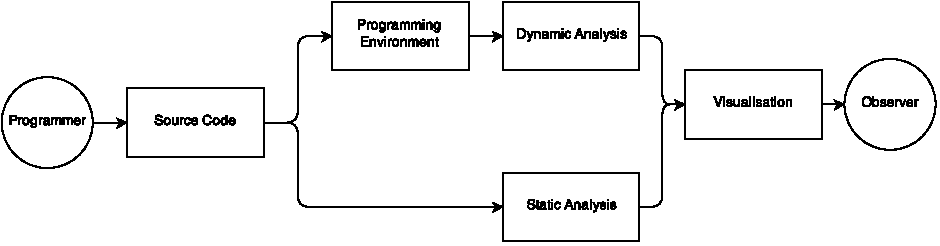
\includegraphics[width=\columnwidth]{../images/diagrams/knowledge-flow-refined.pdf}
  \caption{Knowledge flow from programmer to observer as directed by the visualisation technique employed.}
\label{fig:knowledge-flow-refined}
\end{figure}

Three sources of data were to be combined and visualised including the state of the source code, the state of the running program and the manipulation between the two by the live coder. To achieve this, three major components were required including an application manager, a code manager and an editor plugin (see Figure~\ref{fig:visualisation-class-diagram}). The following sections detail the implementation of these components.

This visualisation was, as with the previous iteration, rendered under the source code. 

% \cite{Heer2006} might be useful for explaining the design of this visualisation...

\begin{figure}
  \centering 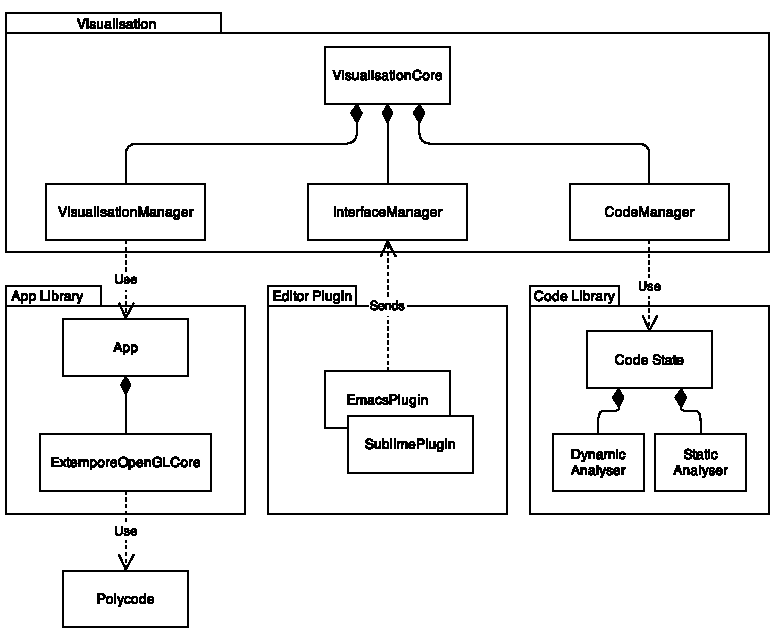
\includegraphics[width=\columnwidth]{../images/diagrams/visualisation-class-diagram.pdf}
  \caption[Prototype (second iteration) class diagram]{Class diagram of the visualisation technique employed. The three major components included the visualisation manager, the interface manager and the code manager.}
\label{fig:visualisation-class-diagram}
\end{figure}

\subsection{Visualisation Manager}

The visualisation manager handled all visual elements on the screen. The Polycode~\cite{Safrin2013} library was bound to the live coding environment allowing for more advanced two-dimensional graphical manipulations than the previous visualisation iteration through scene graph manipulation. Using this technique, the intention was to represent the state of the source code, the manipulation of the source code and the state of the active source code in the same visual environment.

\subsection{Interface Mananger}
\label{sec:interface-manager}

To gather information regarding the actions of the programmer, a method of interfacing with the live coder's programming environment was required. This was acheived using a text editor plugin sending programmer interactions over an \ac{OSC} protocol. The interactions sent included cursor movement, all source code changes, file focus and source code evaluation.

\subsection{Code Manager}

Both static analysis of source code and the dynamic analysis (see~\cite{Eisenbarth2003} and~\cite{Jerding1997}) of the program were combined into this iteration of the visualisation prototype in order to provide the audience with a link between the \acf{SoW} and the \acf{SoC}~\cite{Swift2013}.
% {\color{red} explain what the \ac{SoW} and the \ac{SoC} actually is and show the link between the \ac{SoW} with dynamic analysis and the \ac{SoC} with static analysis...}

Static analysis of the source code involved parsing the changing source code input by the programmer. Data requiring this static analysis was received from the editor plugin (see~\ref{sec:interface-manager}) and stored as the current \ac{SoC}.

Dynamic analysis of the running program involved providing mechanisms for the programmer to send running state information to be stored as the \ac{SoW}. A callback hook was provided to be used when creating an instrument during performance. This hook would provide data on the names of the instruments, the state of the callbacks and would allow links to be determined between the \ac{SoC} and the \ac{SoW}.

\subsection{Mappings}

\begin{figure}
\centering
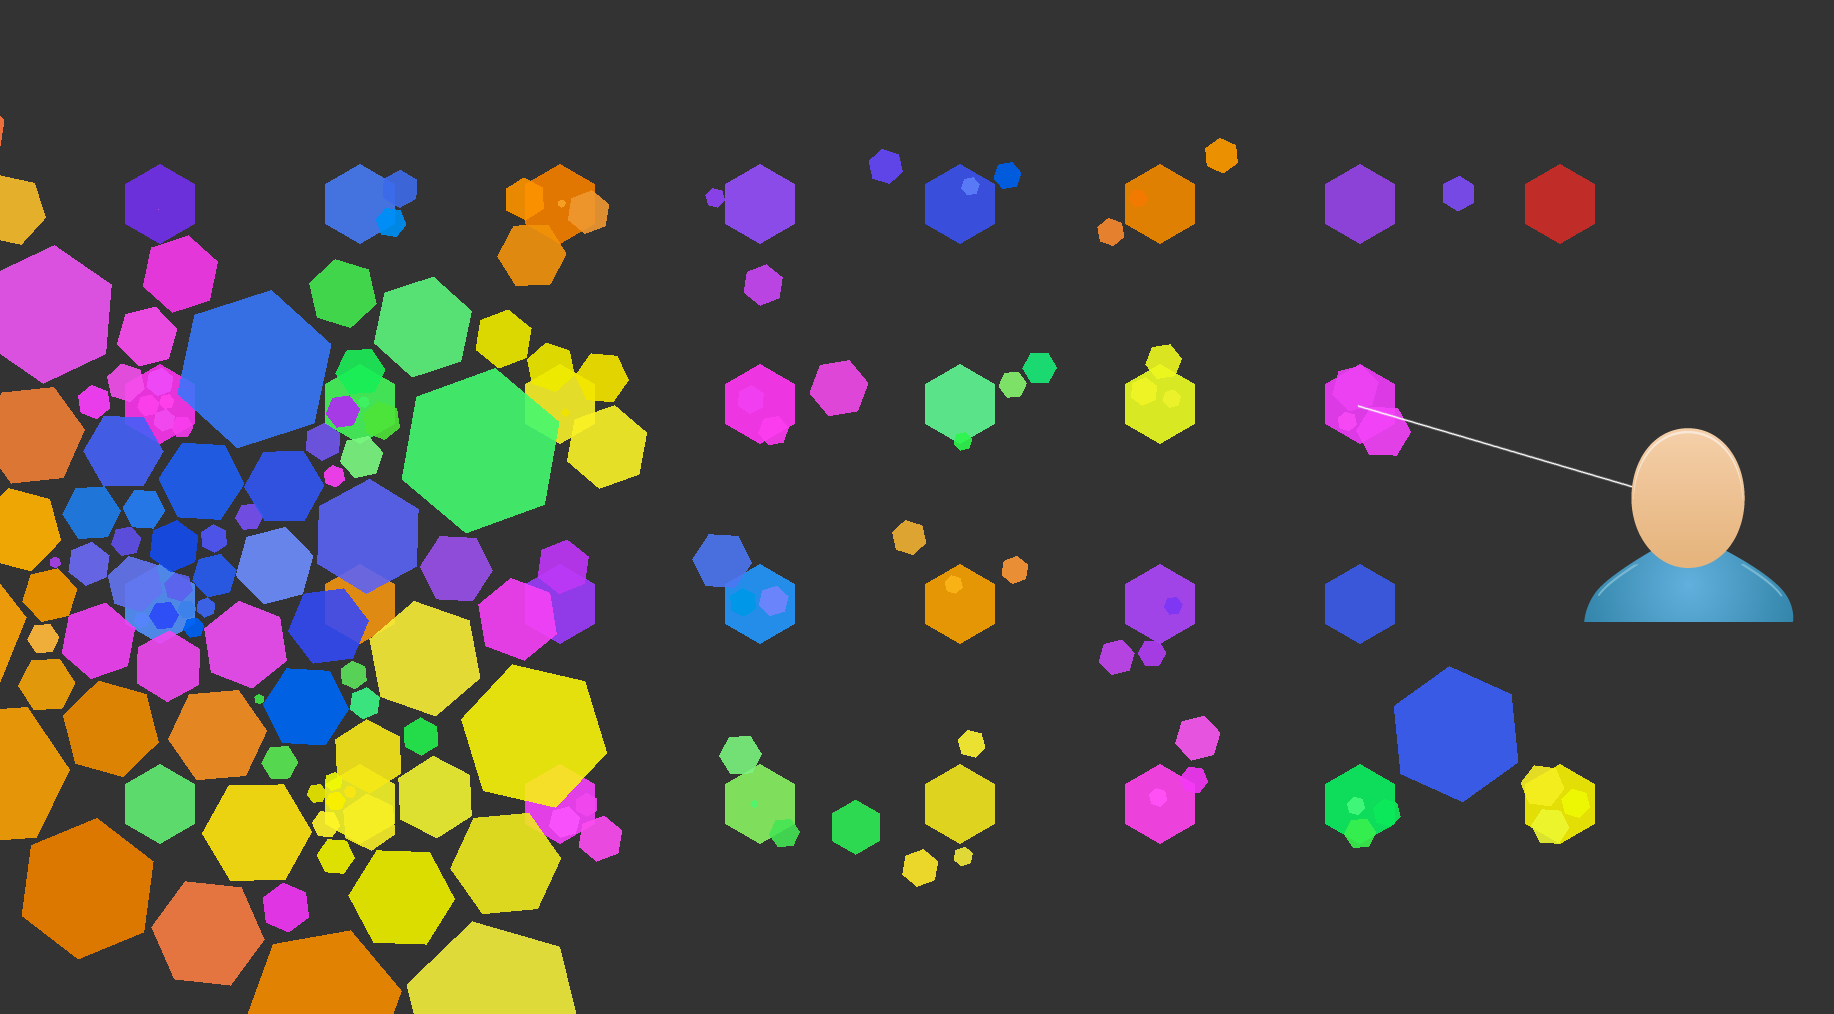
\includegraphics[width=\textwidth]{../images/final-visualisations/final-code-visualisation.png}
\caption[Prototype (second iteration) example]{An example of the visualisation developed.}
\label{fig:final-visualisation}
\end{figure}

A number of specific mappings were assigned to the visualisation. These visual mappings related directly to actions taken by the programmer, behaviour of the running program and representation of the source code. 

Function count was mapped to the number of large visual elements on screen. When adding a new function, a new element was introduced. This mapping was intended to allow the audience to associate the simplified geometric shape to the source code and allow the audience to separate functions visually.

Each large visual element represented the state of active and inactive functions. In live coding, the programmer triggers functions to change between active and inactive states. The mapping represented this though the use of washed out grey and white colours while inactive and vibrant, bright colours while active. In addition, the active functions were animated, with moving visual elements.

Function size and shape was represented visually through the use of ``attractors'' with each line of code mapped to one of the visual elements. Visual elements would grow and shrink according to the length of the line of source code directly mapping the typing actions of the programmer to visual elements.  
% -programmer typing behaviour

% -function beat+callback duration

To ensure the relationship between the actions of the programmer, the changes to the source code and the changes to the music were easily identified, an icon representing the programmer was displayed closest to the function being edited. This mapping intended to provide the audience with a better overview of the movements of the programmer among the functions than would otherwise be visible through the cursor alone.  

% From presentation:

% developed one visualisation taking features from both aesthetic and didactic conditions of the previous user study
% used this to visualise high level code structure and high level live coder actions

% shows:
% state of the active code
% what sections of code are being edited

% -  each hexagon indicates a line of code
% the programmer is shown editing one of the functions
% pulses with the musical output of each function

\section{Development}

A similar approach to the previous iteration of visualisation prototype was taken. This process involved a collaborative approach to development with a live coding artist to develop visualisations appropriate for the live coding context.

\more

The final prototype consisted of approximately 3600 \acf{SLOC}, consisting of 2300 \ac{SLOC} of C++ and C bindings, and 1300 \ac{SLOC} of xtlang.

-discuss reusable infrastructure for static and dynamic code analysis... \more

\subsection{Testing}

\more

Stability was of primary concern during the live performance. To ensure no failures occurred during the live performance, a number of testing strategies were adopted.

Unit testing was carried out on each component.

Integration testing...

System testing...

Finally, evaluation during a user study would act as the acceptance test for the software visualisation method.

\section{Summary}

In summary, this visualisation technique attempted to bring together effective features identified within the aesthetic and didactic visualisations of the previous iteration. The prototype developed included three major components including the visualisation manager, the interface manager and the code manager. Technical limitations with the first iteration of the visualsation prototype were addressed and an attempt was made to communicate the state of the source code, the state of the running program and the manipulation between the two by the live coder. The effectiveness of aligning the mental models of the audience and the live coder was to be evaluated in a follow-up user study.


